\documentclass[a4paper]{article}
\usepackage[utf8]{inputenc}
\usepackage[T1]{fontenc}
\usepackage[frenchb]{babel}
\usepackage{listings}
\usepackage{array}
\usepackage{graphicx}
\usepackage{fullpage}
\title{Equalizator \\ Détection de genre musical par feature-extraction}
\author{}

\begin{document}

\maketitle

\tableofcontents

\newpage

\section{Introduction}

L'une des principales fonctionnalités de notre produit est de pouvoir détecter automatiquement le genre musical d'une chanson
et d'ainsi adapter son égalisation.

Nous avons commencé la réalisation d'un algorithme de détection de genre musical basé sur la \emph{feature extraction} et une régression, des approches typiques du machine learning.

\section{Feature extraction}

\subsection{Idée}

Notre travail est basé sur un article publié en 2001 par l'université de Princeton.

Il s'agit d'analyser le spectre audio des morceaux de musique afin d'en extraire certaines propriétés. Nous avons implémenté le calcul de 5 de ces propriétés, qui sont :

\begin{itemize}

\item Le \emph{Mean-Centroid} mesure de la brillance du spectre audio. Une musique comprenant beaucoup d'aigus et/ou beaucoup d'instruments aura tendance à avoir un \emph{Mean-Centroid} plus élevé

\item Le \emph{Mean-Rolloff} mesure de la répartition du spectre audio. Plus un morceaux contient de basses, plus ce nombre sera grand.

\item Le \emph{Mean-Flux} mesure le "mouvement" dans le spectre audio. Si celui-ci varie rapidement et fréquemment, ce nombre est plus grand.

\item Le \emph{ZeroCross} mesure la quantité de "bruit" d'un morceaux. Un morceau calme aura un \emph{ZeroCross} plus faible.

\item Le \emph{LowEnergy} mesure la quantité de passages dont l'énergie est faible par rapport à la moyenne. Un morceau agité aura un \emph{LowEnergy} faible.


\end{itemize}


On peut ainsi obtenir 5 nombres pour chaque chanson et les classifier en fonction de ceux-ci.

\subsection{Implémentation}

Nous avons utilisé le logiciel libre Scilab. Le code peut être trouvé en Annexe. Nous avons principalement eu recours à la Transformée de Fourier Discrète pour cet algorithme.

Nous avons très rapidement vu de grandes différences dans les propriétés que nous avons extraites de différents morceaux. Les graphiques suivants proviennent des morceaux "Pixel Party" de Vexento et du "Printemps" des 4 saisons de Vivaldi.

\newpage
\begin{figure}[h!]
\begin{center}
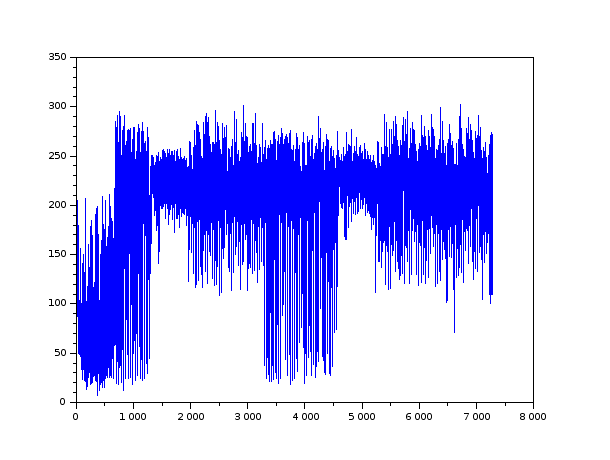
\includegraphics[scale=0.3]{../vexentorolloff.png}
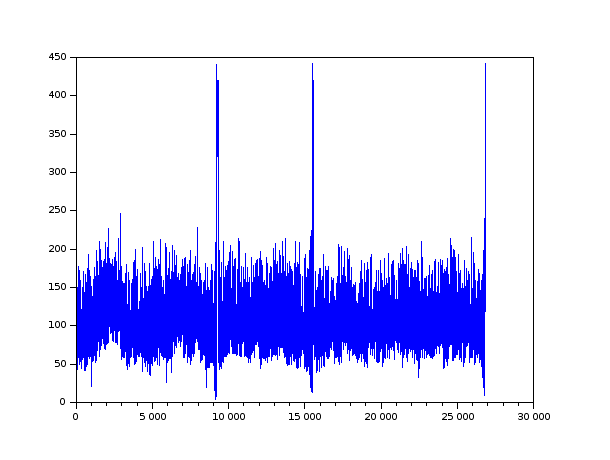
\includegraphics[scale=0.3]{../vivaldirolloff.png}
\caption{Rolloff (quantité de basses) d'un morceau d'electro (à gauche) et d'un morceau de classique (à droite) au cours du temps}
\end{center}
\end{figure}

\begin{figure}[h!]
\begin{center}
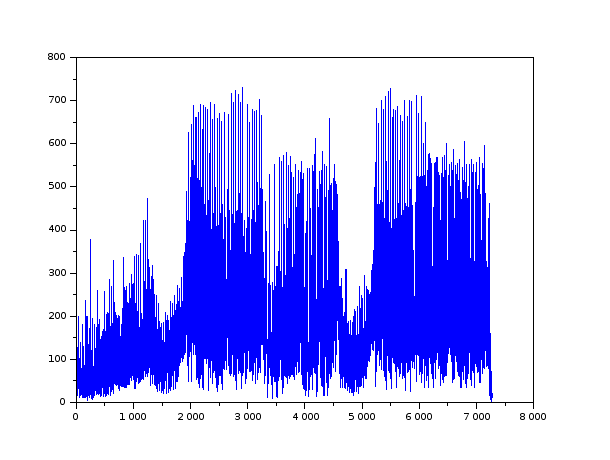
\includegraphics[scale=0.3]{../fluxvexento.png}
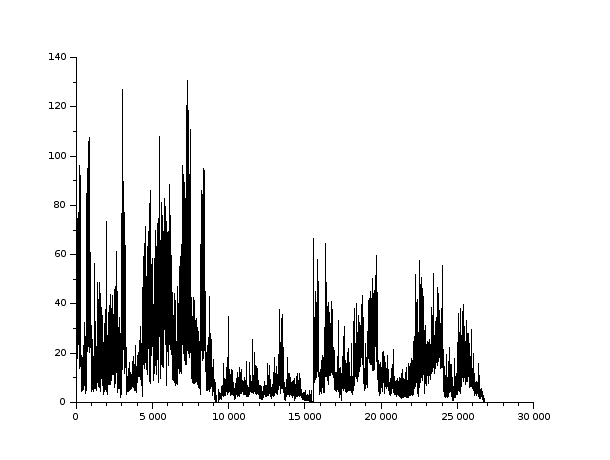
\includegraphics[scale=0.3]{../fluxvivaldi.png}
\caption{Flux (agitation) d'un morceau d'electro (à gauche) et d'un morceau de classique (à droite) au cours du temps}
\end{center}
\end{figure}

\begin{figure}[h!]
\begin{center}
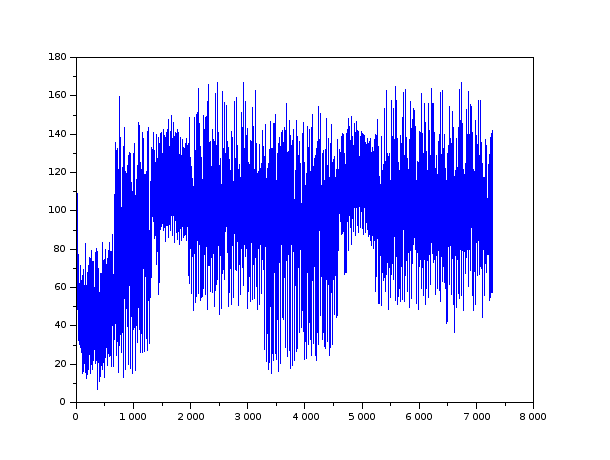
\includegraphics[scale=0.3]{../vexentocentroid.png}
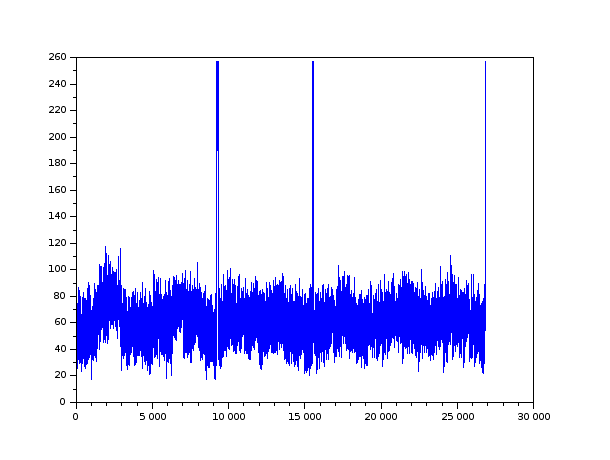
\includegraphics[scale=0.3]{../vivaldicentroid.png}
\caption{Centroide (brillance) d'un morceau d'electro (à gauche) et d'un morceau de classique (à droite) au cours du temps}
\end{center}
\end{figure}
\newpage


\subsection{Résultats}

Voici les résultats que nous avons obtenus pour 4 morceaux. 2 morceaux de musique classique (Vivaldi, Haendel) et 2 morceaux de musique électronique (AdhesiveWombat, Vexento).

\begin{center}
\begin{tabular}{|l|l|l|l|l|l|}
\hline
      Titre     & Centroid & Rolloff & Flux & ZeroCross & LowEnergy \\
      \hline
 Pixel Party   & 92.3  & 195.3 & 173.2 & 81.3 & 52\% \\
 8-bit Adventure  & 94.2 & 205.6 & 108.9 & 80.7 & 48\% \\ 
 \hline
 4 saisons, Printemps  & 59.2 & 98.8 & 15.7 & 58.0 & 62\% \\
 Water Music 1 Haendel  & 55.7 & 90.7 & 23.4 & 54.6 & 61\% \\
 \hline
\end{tabular}
\end{center}

On peut voir de nettes différences entre les chiffres des deux genres musicaux. On voit également qu'au sein d'un genre musical, les chiffres se ressemblent.


\section{Régression logistique}

\subsection{Principe}

N'ayant pas énormément de temps pour analyser beaucoup de fichiers audio, nous avons décidé de faire notre régression logistique sur les 4 morceaux qui ont été analysés ci-dessus. On définit avec les nombres obtenus un espace à 5 dimensions auquel on ajoute une dimension pour des scores arbitraires qu'on attribue à chaque genre.

À l'aide du tableau ci-dessus, on crée une matrice $X$ contenant les résultats obtenus. On décide d'assigner aux morceaux de classique le score $1$, et aux morceaux d'électro le score $0$. Ce qui nous donne le vecteur $p = (1,1,0,0)$.

Il s'agit maintenant de trouver un vecteur $a$ et un scalaire $b$ vérifiant : $log(\frac{p}{1-p}) = Xa +b$.

On fait cela à l'aide de la fonction \emph{glm} de R (cf Annexe 2).

Et on obtient : 

$a = (-2.22428 ,0.41626 ,-0.08565 ,0.59464 ,1.57771)$ et $b = -15.78057$.

\subsection{Exploitation}

On décide pour valider notre algorithme d'analyser pour 4 morceaux différents de ceux que nous avons utilisé pour créer notre modèle. On analyse ici dix secondes de musique, et non pas l'intégralité des morceaux comme précédemment.

Les morceaux utilisés sont :

\begin{itemize}

\item 2e mouvement de la Sonate au clair de lune de Beethoven
\item une sonate de Chopin
\item Force - Alan Walker
\item Unity - TheFatRat

\end{itemize}

On choisit les dix secondes étudiées arbitrairement dans les morceaux (ici on a choisi de les prendre au milieu du morceau). On fait la même analyse que précédemment, on obtient donc 5 chiffres représentant ces dix secondes, qu'on stocke dans un vecteur $x$, puis qu'on remplace dans $ y = a*x + b$. On a ensuite $p = \frac{e^{y}}{1+e^{y}}$. Ce qui nous donne $p$, la probabilité qu'un morceau soit de la musique classique. 

\subsection{Résultats}

Quand $y$ est proche de 1, on dit que le morceau est "classique", quand $y$ est proche de 0, on dit que le morceau est "electro". Notre algorithme a réussi a trouver le genre des 4 morceaux énoncés ci-dessus.

\newpage

\section{Annexes}
\subsection{Programme d'analyse}
\lstinputlisting[frame = single, language = Scilab,breaklines=true, basicstyle=\footnotesize\ttfamily ]{../analysis.sce}

\subsection{Regression logistique}
\lstinputlisting[frame = single,breaklines=true, basicstyle=\footnotesize\ttfamily ]{../logit.R}

\subsection{Fonction de prédiction}
\lstinputlisting[frame = single, language = Scilab,breaklines=true, basicstyle=\footnotesize\ttfamily ]{../predict.sce}




\end{document}
